\section{Implementering af DSP modul}\label{sec:implementering_dsp}
DSP modulet har til opgave at beregne koefficienter, beregne amplitude (til lcd'en), udføre det 
digitale filter på de samples der modtages mm.. På figur \ref{fig:dsp_flow_diag} illuteres data flow'et 
som kommunikerer med equalizer modulet.

\begin{figure}[h]
\centering
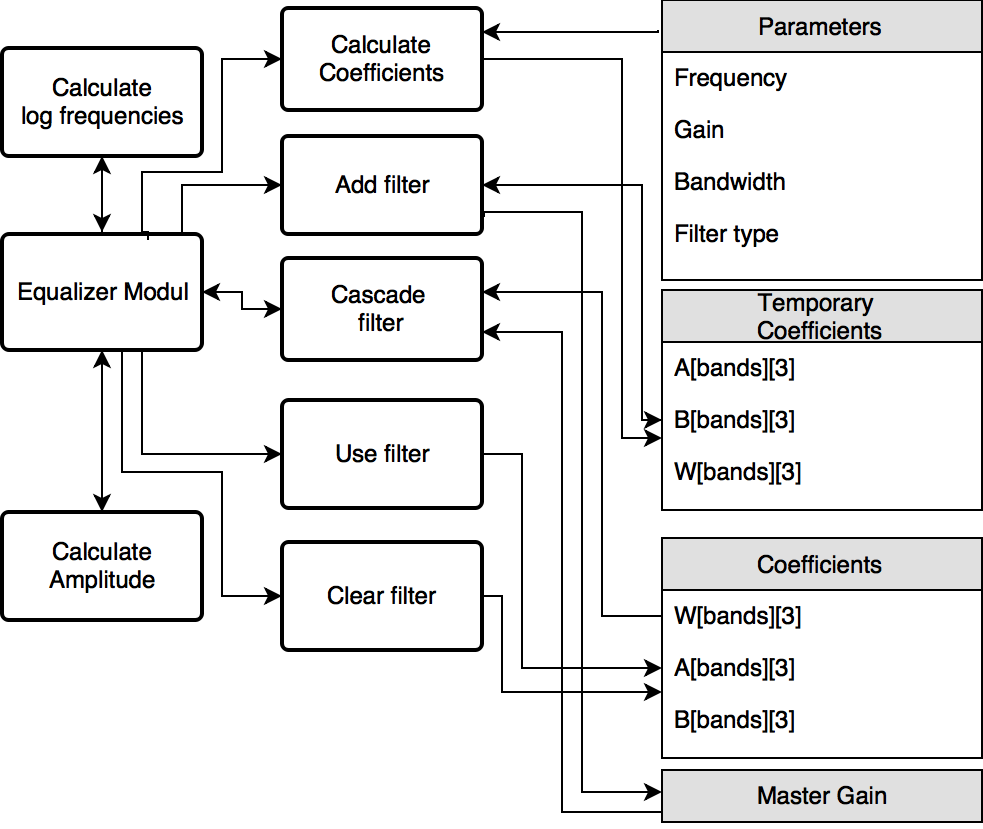
\includegraphics[scale = 0.3]{billeder/dsp_flowdiagram}
\caption{Flowdiagram af dsp modulet.}
\label{fig:dsp_flow_diag}
\end{figure}


beregning af amplitude \\
beregning af coefficienter\\
add filter \\
use filter \\
clear filter \\
cascade filter \\
